\chapter{微分方程和差分方程}

微分方程和差分方程是在时域描述系统的典型方法。
本章讲述微分方程、差分方程和通过欧拉近似将微分方程转为差分方程求得数值解。

微分方程是描述系统的最基础的方法,直接由物理公式推导得到,也是最接近物理本质的方法。
差分方程可以理解为一种求解微分方程数值解的方法。

本章要点:
\begin{itemize}
    \item LTI系统的微分方程。
    \item LTI系统的差分方程。
    \item 微分方程的离散化。
\end{itemize}

\newpage
\section{LTI系统的微分方程模型}

很多物理系统,如电路、钟摆、悬挂等,其变量间存在导数和积分关系,整个系统可用微分方程描述,所以微分方程模型关键在于建模和求解微分方程。

本节要点:
\begin{itemize}
    \item 掌握微分方程的概念;
    \item 掌握一阶常系数线性微分方程的求解思路。
\end{itemize}

%============================================================
\subsection{微分方程的概述}

若LTI系统是有限维度,则可以用线性常系数微分方程描述如下:
\[
y^{\left( n \right)}\left( t \right) +\sum_{i=0}^{n-1}{A_iy^{\left( i \right)}\left( t \right)}=\sum_{i=0}^m{B_ix^{\left( i \right)}\left( t \right)}
\]
其中,$A_i,B_i$是实数,$n$称为{\bf 系统的阶}(order)。
配合初始条件,即可求出输入输出的对应关系。
特别地,我们称
\[
y\left( t \right) =B_0x\left( t \right)
\]
这样的系统为{\bf 静态系统},即输出只与当刻的输入有关。
静态系统过于简单,不予讨论。
如果系统的输出不仅与当刻输入有关,更与前刻输入有关,则称为{\bf 动态系统},动态系统的时域模型必为微分方程。
通常简单的微分方程可以求解,复杂的方程非常难解,特别是高阶的,甚至没有解析解。

一般来讲,真实系统多多少少都会将输入信号的能量在系统内部有暂留,相当于输出的能量在系统内部“来回振荡”了几下叠合起来再输出,所以在时域模型上,都会体现成微分方程,至少是一阶。

%============================================================
\subsection{一阶常系数线性方程的求解}

\begin{tcolorbox}
为了方便求解,时域分析(本章和下一章的卷积)的大量例子都是以一阶微分方程为例,所以这里特别讨论一阶常系数线性方程的求解方法。
微积分中的一阶常系数线性微分方程是关于一元函数$y=y\left( x \right) $的方程。
信号与系统中不一样,同样是一元函数,但是是$t$的参数方程$x=x\left( t \right) ,y=y\left( t \right) $。
\end{tcolorbox}

考虑如下形式的微分方程(一阶、常系数、非齐次):
\[
\frac{dy}{dt}+Py=Qx \qquad t\geqslant t_0
\]
\begin{itemize}
    \item $x=x\left( t \right) ,y=y\left( t \right) $:时间$t$的函数,表示输入信号和输出信号;
    \item $P,Q$:常实数。
\end{itemize}

采用变量替换法求解,首先两边同乘系数$e^{Pt}$:
\begin{align*}
&\because e^{Pt}\left( \frac{dy}{dt}+Py \right) =e^{Pt}Qx \\
&\therefore \frac{d}{dt}\left( e^{Pt}y \right) =Q\left( e^{Pt}x \right)
\end{align*}
变量替换$Y=e^{Pt}y,X=e^{Pt}x$,解得:
\begin{align*}
&\frac{d}{dt}Y=QX \\
&Y=Y\left( t_0 \right) +Q\int_{t_0}^t{Xd\tau}
\end{align*}
替换回,最终得到一阶微分方程的通解:
\begin{align*}
y\left( t \right) &=e^{-P\left( t-t_0 \right)}y\left( t_0 \right) +Qe^{-Pt}\int_{t_0}^t{e^{P\tau}x\left( \tau \right) d\tau} \qquad t\geqslant 0 \\
&=e^{-Pt}\left[ e^{Pt_0}y\left( t_0 \right) +Q\int_{t_0}^t{e^{P\tau}x\left( \tau \right) d\tau} \right]
\end{align*}
输出由两部分组成:
\begin{itemize}
    \item $e^{-Pt}e^{Pt_0}y\left( t_0 \right) $:对初始条件的响应,呈指数形式衰减;
    \item $e^{-Pt}Q\int_{t_0}^t{e^{P\tau}x\left( \tau \right) d\tau}$:对输入的响应,具体需要看输入的形式,但同样也是呈指数形式衰减。
\end{itemize}

%============================================================
\subsection{例RC电路}

\begin{example}
如下电路,假设系统零状态,若输入为单位阶跃信号$x=u\left( t \right) $,求系统的输出。
\end{example}

\begin{figure}[h]
\centering
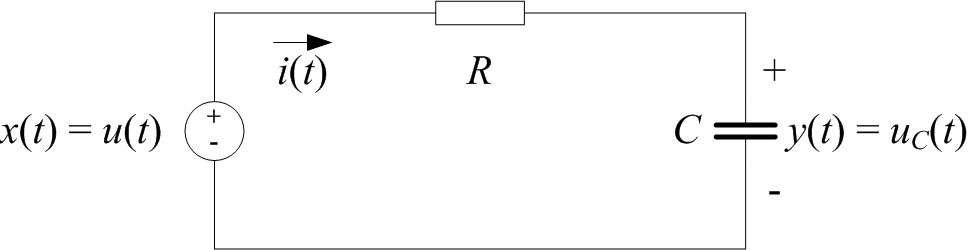
\includegraphics[height=2cm]{1.5.1-1.png}
\end{figure}

根据之前的分析,系统的微分方程模型:
\[
\frac{dy}{dt}+\frac{1}{RC}y=\frac{1}{RC}x \qquad \begin{cases}
	x\left( t \right) =u\left( t \right)\\
	y\left( 0^- \right) =0\\
\end{cases}
\]
求解该微分方程得到输出信号:
\begin{align*}
y\left( t \right) &=e^{-Pt}\left[ e^{Pt_0}y\left( t_0 \right) +Q\int_{t_0}^t{e^{P\tau}x\left( \tau \right) d\tau} \right] \\
&=e^{-\frac{1}{RC}t}\left[ y\left( 0 \right) +\frac{1}{RC}\int_0^t{e^{\frac{1}{RC}\tau}u\left( \tau \right) d\tau} \right] \\
&=\frac{1}{RC}e^{-\frac{1}{RC}t}\left[ \int_0^t{e^{\frac{1}{RC}\tau}d\tau} \right] =\frac{1}{RC}e^{-\frac{1}{RC}t}\left[ \left. RCe^{\frac{1}{RC}\tau} \right|_{0}^{t} \right] \\
&=1-e^{-\frac{t}{RC}} \qquad t\geqslant 0
\end{align*}
画图如下,可见,减小电阻或电容都可以提高输出对输入的“跟随性”。

\begin{python}
t  = np.arange(0, 10, 0.01)
RC = 1;   y1 = 1 - np.exp(-1 * t / RC)
RC = 0.1; y2 = 1 - np.exp(-1 * t / RC)

ax.plot(t, y1,       label='RC=1')
ax.plot(t, y2, '--', label='RC=0.1')
\end{python}

\begin{figure}[h]
\centering
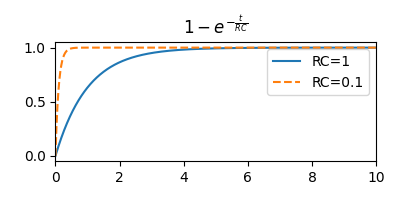
\includegraphics[height=3cm]{2.1.3-1.png}
\end{figure}






\newpage
\section{LTI系统的差分方程模型}

本节讨论离散系统的差分方程模型。

本节要点:
\begin{itemize}
    \item 掌握差分方程的概念;
    \item 理解差分方程的物理意义;
    \item 掌握差分方程的求解思路;
    \item 编写Python函数求解n阶线性常系数差分方程。
\end{itemize}

%============================================================
\subsection{差分方程的概念}

如果离散LTI系统有限维度,可以用线性常系数差分方程描述如下:
\[
y\left[ n \right] +\sum_{i=1}^N{A_iy\left[ n-i \right]}=\sum_{i=0}^M{B_ix\left[ n-i \right]}
\]
即系统某刻的输出$y\left[ n \right] $,由此刻的输入$x\left[ n \right] $和之前的输入$x\left[ n-i \right] $和之前的输出$y\left[ n-i \right] $,一共$N+M+1$个量共同决定。
通常配合初始条件,通过递归计算的方法就可以解出$y\left[ n \right] $。
这样的系统称为{\bf 递归型离散系统}(recursive discrete-time system)或{\bf 递归型数字滤波器}(recursive digital filter)。

%============================================================
\subsection{差分方程的物理意义}

以一阶差分方程为例:
\[
y\left[ n \right] +Ay\left[ n-1 \right] =Bx\left[ n \right]
\]
表示系统当刻输出$y\left[ n \right] $是当刻输入$x\left[ n \right] $和前刻输出$y\left[ n-1 \right] $的线性叠加。

这里要注意:
\begin{itemize}
    \item $B$:对系统稳定性来讲没有任何关系,只是表明系统是放大器还是衰减器;
    \item $y\left[ n-1 \right] $:表示系统内部对能量的回响;
    \item $A$:表示这种回响以反馈的方式造成混响,决定了系统的稳定性。
\end{itemize}
还要特别注意,这种回响不是一次性的,它造成的叠加输出在后一刻继续以混响的方式反馈于系统。
如果系统是LTI,则这种回响是关于时间的一个等比数列,造成的混响就是这个等比数列的和。

%============================================================
\subsection{一阶差分方程的求解}

对于一阶差分方程$y\left[ n \right] +Ay\left[ n-1 \right] =Bx\left[ n \right] $,可以通过不断递归求解,这里直接给出解:
\[
y\left[ n \right] =\left( -A \right) ^ny\left[ 0 \right] +\sum_{i=1}^n{\left( -A \right) ^{n-1}Bx\left[ i \right]} \qquad n=1,2,\cdots
\]

%============================================================
\subsection{Python应用——n阶差分方程的实现}

这里,我们编写一个Python函数(my\_diff)用以求解n阶差分方程:
\[
y\left[ n \right] +\sum_{i=1}^N{A_iy\left[ n-i \right]}=B_0x\left[ n \right] +\sum_{i=1}^M{B_ix\left[ n-i \right]}
\]

已知(同时也是函数的参数):
\begin{itemize}
    \item 系数(按照差分方程的系数排序):
    \[
    A_1,A_2,\cdots ,A_N,B_0,B_1,B_2,\cdots ,B_M
    \]
    \item 初始条件(按时间从最远点到最近点排序):
    \[
    y\left[ -N \right] ,\cdots ,y\left[ -1 \right] ,x\left[ -M \right] ,\cdots ,x\left[ -1 \right]
    \]
    \item 输入信号序列:
    \[
    x\left[ 1 \right] ,x\left[ 2 \right] ,\cdots ,x\left[ n \right]
    \]
\end{itemize}
取$y\left[ 1 \right] ,y\left[ 2 \right] $观察:
\begin{align*}
y\left[ 1 \right] =&A_1y\left[ -N \right] +A_2y\left[ -N+1 \right] \cdots A_{N-1}y\left[ -2 \right] +A_Ny\left[ -1 \right] + \\
&B_1x\left[ -M \right] +B_2x\left[ -M+1 \right] \cdots B_{M-1}x\left[ -2 \right] +B_Mx\left[ -1 \right] + \\
&Bx\left[ 1 \right] \\
y\left[ 2 \right] =&A_1y\left[ -N+1 \right] +A_2y\left[ -N+2 \right] \cdots A_{N-1}y\left[ -1 \right] +A_Ny\left[ 1 \right] + \\
&B_1x\left[ -M+1 \right] +B_2x\left[ -M+2 \right] \cdots B_{M-1}x\left[ -1 \right] +B_Mx\left[ 1 \right] + \\
&Bx\left[ 2 \right]
\end{align*}

设计参数:
\begin{itemize}
    \item An:$N$维向量,表示$A_1,A_2,\cdots ,A_N$;
    \item Yn:$N$维向量,表示输出信号的初始值$y\left[ -1 \right] ,y\left[ -2 \right] ,\cdots ,y\left[ -N \right] $;
    \item Bm:$M$维向量,表示$B_1,B_2,\cdots ,B_M$;
    \item Xm:$M$维向量,表示输入信号的初始值$x\left[ -1 \right] ,x\left[ -2 \right] ,\cdots ,x\left[ -M \right] $;
    \item b:标量,表示$B_0$;
    \item X:表示输入信号$x\left[ 1 \right] ,x\left[ 2 \right] ,\cdots ,x\left[ n \right] $。
\end{itemize}

过程注解:
\begin{enumerate}
    \item 将Yn和Xm翻转,以匹配An和Bm;
    \item 构造输出Y,和X一样长度,填充0;
    \item 计算每个Y[i],期间更新Yn和Xm;
    \item 返回Y。
\end{enumerate}

注意:
\begin{itemize}
    \item An和Yn的长度必须一致;
    \item Bm和Xm的长度必须一致;
    \item b是标量;
    \item 最终输出信号Y的长度由输入信号X决定。
\end{itemize}

\begin{python}
def my_diff(
        An:np.ndarray, Yn:np.ndarray,
        Bm:np.ndarray, Xm:np.ndarray,
        b:float,
        X:np.ndarray
        ) -> np.ndarray:

    Yn = np.flipud(Yn)
    Xm = np.flipud(Xm)
    Y  = np.zeros_like(X)

    for i in range(X.shape[0]):
        Y[i] = b*X[i] + np.dot(Bm, Xm) - np.dot(An, Yn)
        Yn = np.append(Yn, Y[i])[1:]
        Xm = np.append(Xm, X[i])[1:]
        pass

    return Y
\end{python}






\newpage
\section{微分方程的离散化}

对于不容易求解的微分方程,比如高阶方程,可以通过对时间的离散化变成差分方程,再通过递归获得数值解。

本节要点:
\begin{itemize}
    \item 掌握欧拉近似方法。
\end{itemize}

%============================================================
\subsection{一阶微分方程的欧拉近似}

一阶常系数微分方程:
\[
\frac{dy}{dt}+Py=Qx \qquad t\geqslant t_0
\]
假设时间取离散点$t=nT$,则:
\[
\frac{dy\left( nT \right)}{d\left( nT \right)}+Py\left( nT \right) =Qx\left( nT \right) \qquad n=0,1,2,\cdots
\]
如果采样周期足够小,方程左边可以认为$\frac{1}{T}\left[ y\left( nT+T \right) -y\left( nT \right) \right] +Py\left( nT \right) $,于是一阶微分方程可以离散地表示为:
\[
y\left[ n \right] +\left( PT-1 \right) y\left[ n-1 \right] =TQx\left[ n-1 \right] \qquad n=0,1,2,\cdots
\]
该一阶差分方程即为一阶微分方程的近似,根据之前讨论的方法即可得到采样点的输出信号,该过程称为{\bf 欧拉近似}(Euler approximation)。
欧拉近似是一种对微分方程数值化求解的方法,采样周期越小,精度越高。

%============================================================
\subsection{二阶微分方程的欧拉近似}

对于二阶微分方程:
\[
\frac{d^2y}{dt^2}+A_1\frac{dy}{dt}+A_0y=B_1\frac{dx}{dt}+B_0x \qquad t\geqslant t_0
\]
用欧拉近似可得差分方程:
\begin{align*}
&\frac{y\left[ n \right] +y\left[ n-2 \right]}{T^2}+A_1\frac{y\left[ n-1 \right] -y\left[ n-2 \right]}{T}+A_0y\left[ n-2 \right] \\
&=B_1\frac{x\left[ n-1 \right] -x\left[ n-2 \right]}{T}+B_0x\left[ n-2 \right]
\end{align*}
整理后:
\begin{align*}
&y\left[ n \right] +\left( A_1T-2 \right) y\left[ n-1 \right] +\left( A_0T^2-A_1T+1 \right) y\left[ n-2 \right] \\
&=B_1Tx\left[ n-1 \right] +\left( B_0T^2-B_1T \right) x\left[ n-2 \right]
\end{align*}

%============================================================
\subsection{例RC电路}

\begin{example}
以下图为例,假设电路零状态,$x\left( t \right) =1\mathrm{V},R=1\Omega ,C=1\mathrm{F}$,分别用微分方程和差分方程计算系统在0~10s这段时间内的输出。
\end{example}

\begin{figure}[h]
\centering
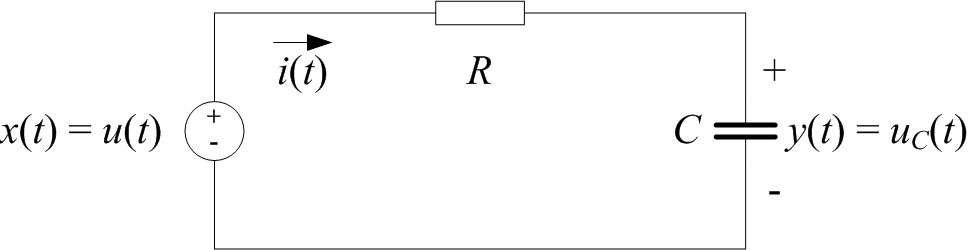
\includegraphics[height=2cm]{1.5.1-1.png}
\end{figure}
\[
\frac{dy}{dt}+\frac{1}{RC}y=\frac{1}{RC}x \qquad \begin{cases}
	x\left( t \right) =u\left( t \right)\\
	y\left( 0^- \right) =0\\
\end{cases}
\]

将之前的结果解得到输出信号并将其做欧拉近似得到差分方程:
\begin{align*}
&y\left( t \right) =1-e^{-\frac{t}{RC}}=1-e^{-t} \qquad t\geqslant 0 \\
&y\left[ n \right] +\left( T-1 \right) y\left[ n-1 \right] =Tx\left[ n-1 \right] \qquad n=0,1,2,\cdots
\end{align*}
令采样间隔$T=0.2\mathrm{s}$,微分方程和差分方程结果如下。

\begin{python}
T  = 0.2
An = np.array([T-1])
Bm = np.array([T])
b  = 0
Yn = np.array([0])
Xm = np.array([0])
t  = np.arange(0, 10, T)
X  = np.ones_like(t)
Y_differential = 1 - np.exp(-1*t)
Y_difference   = my_diff(An, Yn, Bm, Xm, b, X)

ax.plot(t, Y_differential,      label='differential')
ax.plot(t, Y_difference,   'o', label='difference')
\end{python}

\begin{figure}[h]
\centering
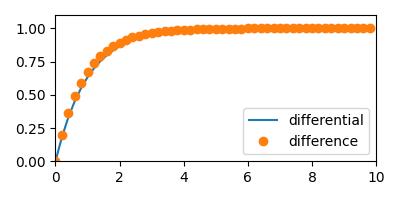
\includegraphics[height=3cm]{2.3.3-1.png}
\end{figure}






\newpage
\section{本章小结}

本章介绍了有限维度LTI系统的两种模型,微分方程模型和差分方程模型。

微分方程模型是最基本、最直观的物理模型。
由于本书只从信号与系统的角度阐述微分方程,所以建议与微积分中的微分方程章节,和选一门工科基础课程(如电路原理)中的微分方程章节,一起相互印证学习。

差分方程模型是微分方程模型的数值化计算,主要掌握离散化方法即可。









